\section{System Exploration and Findings}

This section summarizes the exploration process, focusing on understanding the structure, tables, and solutions used in the NBS system.

\subsection{Overview}

To fully understand the current state of the system, an exploration of its structure, components, and data was conducted. This section provides an in-depth look at the findings from the exploration, focusing on tables, solutions, and Power BI reports that make up the system.

The exploration began with an analysis of tables within NBS. They were examined to understand their structure, the relationships between them, and the quality of the data they contain. Additionally, the system's solutions were reviewed and listed.

Furthermore, the exploration included a review of the Power BI reports used to visualize the data. Along with tables and solutions, these reports were also comprehensively inventorized.

This section includes a detailed inventory of the tables, solutions, and reports. These findings serve as the foundation for the subsequent analysis, providing a clear picture of the NBS components.

\subsection{Tables}

The tables used in the NBS system are referred to as "entities." In the Microsoft Dataverse structure, each entity has a logical name (the actual name of the entity) as well as a display name, which is user-friendly and displayed in the application frontend.

While exploring the system, it appeared that tables related to NBS often start with one of the following prefixes: \texttt{cr675\_}, \texttt{cr91b\_}, or \texttt{craab\_}. As the Microsoft Dataverse API returns a list of all tables, these prefixes served as flags when identifying which tables could be related to NBS. This approach narrowed down the search from hundreds of tables to several dozen.

Another indication of which tables were in use was the \texttt{Data Analyzer} Power BI report.

\newpage

\subsubsection{List of Tables}

This is a list of tables used by NBS. The end user will probably recognize the tables by their display name; however, when programmatically exploring the data, the logical name is used to identify tables.

\begin{footnotesize}
	\begin{tabularx}{\textwidth}{l|l}
		\textbf{Display Name} & \textbf{Logical Name} \\\hline\\
		\textbf{NBS Test Action} & \texttt{cr675\_testdashboardtestprocedment} \\[0.5em]
		\textbf{IFS MATERIALS V3} & \texttt{cr675\_ifsmaterialsv3} \\[0.5em]
		\textbf{NBS Construction Material Stacks Stitchings} & \texttt{cr675\_nbsconstructionmaterialstacksstitchings} \\[0.5em]
		\textbf{NBS IFS MATERIALS} & \texttt{cr675\_nbsifsmaterials} \\[0.5em]
		\textbf{NBS Material stack} & \texttt{cr675\_nbsmaterialstack} \\[0.5em]
		\textbf{NBS Sample} & \texttt{cr675\_testdashboardsample} \\[0.5em]
		\textbf{NBS Test Compound} & \texttt{cr675\_testcompounds} \\[0.5em]
		\textbf{NBS Test Order} & \texttt{cr675\_testorder} \\[0.5em]
		\textbf{NBS ICW Products} & \texttt{cr675\_nbsicwproducts} \\[0.5em]
		\textbf{NBS R Table} & \texttt{cr91b\_nbsrtable} \\[0.5em]
		\textbf{NBS Ballistic System} & \texttt{cr675\_testdashboardballisticsystem} \\[0.5em]
		\textbf{NBS Construction} & \texttt{cr675\_nbsconstruction} \\[0.5em]
		\textbf{NBS Product} & \texttt{cr675\_testdashboardproduct} \\[0.5em]
		\textbf{NBS FREC2 RND Orders} & \texttt{cr675\_nbsfrec2rndorders} \\[0.5em]
		\textbf{NBS Operation} & \texttt{cr675\_nbsstitching} \\[0.5em]
		\textbf{NBS Material} & \texttt{cr675\_nbsmaterial} \\[0.5em]
		\textbf{NBS Test Protocol Template} & \texttt{cr675\_testdashboardstandarddetails} \\[0.5em]
		\textbf{NBS Bullet Type Dictionary} & \texttt{cr675\_testdashboardammotypedictionary} \\[0.5em]
		\textbf{NBS Project} & \texttt{cr675\_project} \\[0.5em]
		\textbf{NBS Geometry} & \texttt{cr675\_testdashboardgeometries} \\[0.5em]
		\textbf{NBS Group Order} & \texttt{craab\_nbsgrouporder} \\[0.5em]
		\textbf{NBS MaterialStackAndConstraction} & \texttt{cr675\_nbsmaterialstackandconstraction} \\[0.5em]
		\textbf{NBS Program} & \texttt{cr91b\_nbsprogram} \\[0.5em]
		\textbf{NBS Standard Names Dictionary} & \texttt{cr675\_testdashboardstandard} \\[0.5em]
		\textbf{NBS Preliminary Testing} & \texttt{cr675\_nbspreliminarytesting} \\[0.5em]
		\textbf{NBS Backing Type Dictionary} & \texttt{cr675\_nbstestdashboardbackingtypedictionary} \\[0.5em]
		\textbf{NBS Cartridge Type Dictionary} & \texttt{cr675\_nbstestdashboardcartridgetypedictionary} \\[0.5em]
		\textbf{NBS Institute} & \texttt{cr675\_testdashboardinstitute} \\[0.5em]
		\textbf{R\&DOrderView} & \texttt{cr675\_orderviewrd} \\[0.5em]
		\textbf{NBS FRECII Tool Type} & \texttt{craab\_nbstooltype} \\[0.5em]
		\textbf{NBS Powder Type Dictionary} & \texttt{cr675\_nbstestdashboardpowdertypedictionary} \\[0.5em]
		\textbf{NBS Photo} & \texttt{cr675\_testdashboardphotos} \\[0.5em]
	\end{tabularx}
\end{footnotesize}

\subsubsection{Entity Relationship Diagram}

This is the Entity Relationship Diagram of the main tables used in NBS. It provides a clear picture of the relationships between tables and can serve as a suggestion for which tables should be merged while preparing data for analysis.

\begin{figure}[h!]
\centering
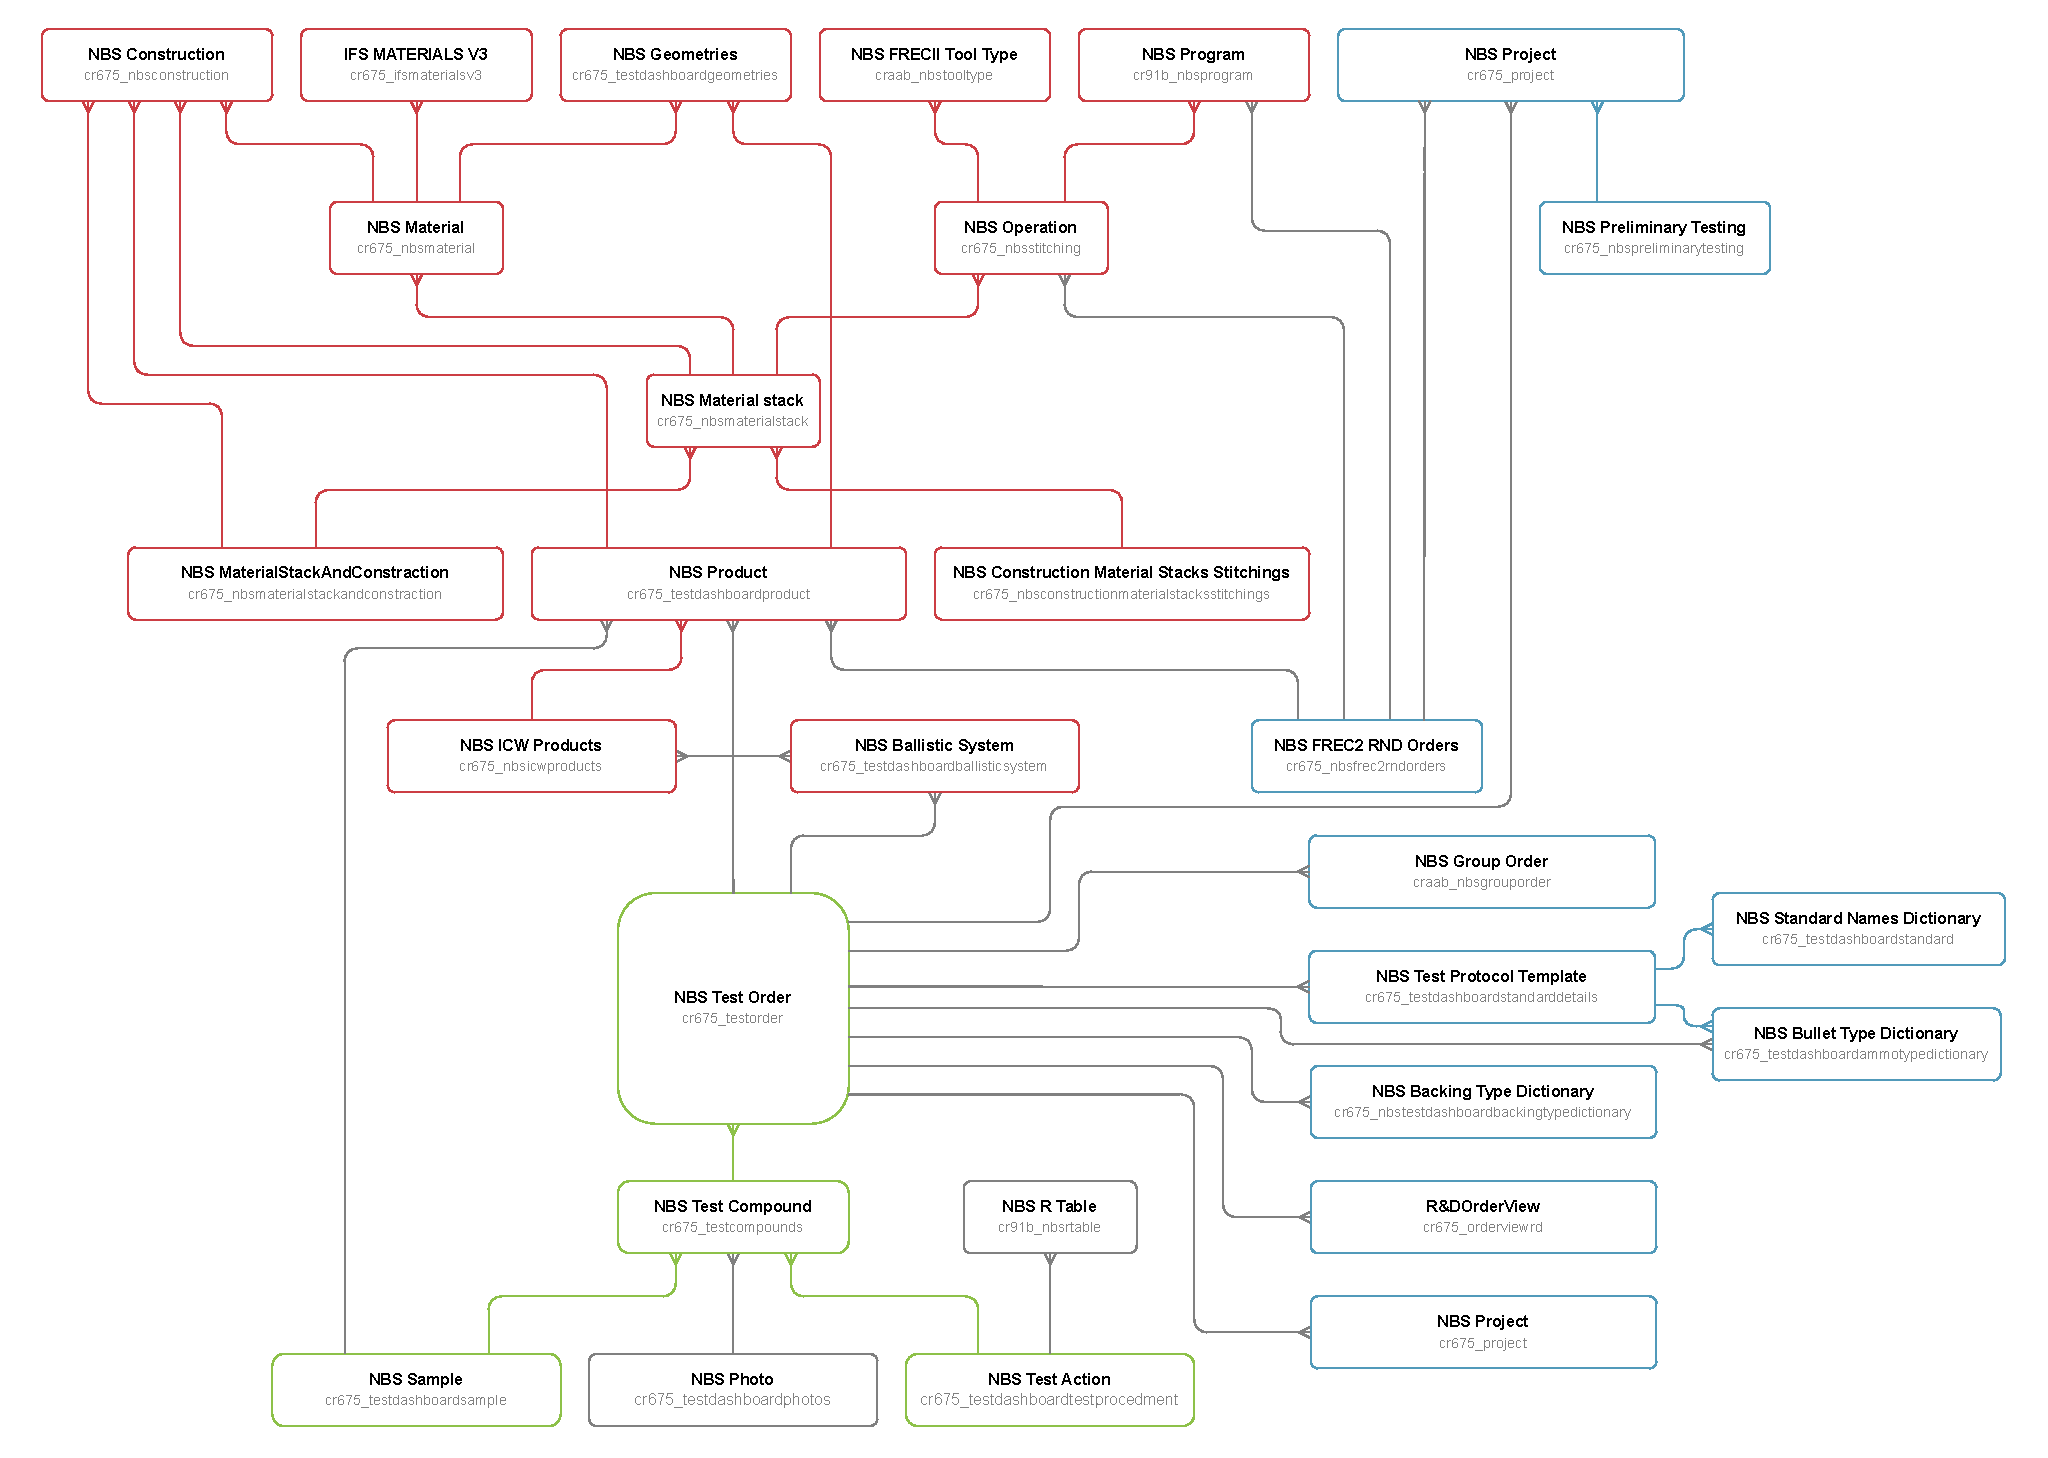
\includegraphics[width=\textwidth]{PDFs/er_diagram.pdf}
\end{figure}

The diagram uses Barker's Notation for entity relationships. For reference see \href{https://ece.uprm.edu/~icom5047/documents/barkers-erd-notation.pdf}{Barker's ERD Notation}

Colors used in the diagram are used for logical grouping of tables:
\begin{itemize}
    \item Tables related to \textcolor[HTML]{cc3e44}{materials/constructions} are highlighted in \textcolor[HTML]{cc3e44}{red}.
    \item Tables related to \textcolor[HTML]{8dc149}{tests} are highlighted in \textcolor[HTML]{8dc149}{green}.
    \item Tables which serve as \textcolor[HTML]{519aba}{dictionaries/indexes} are highlighted in \textcolor[HTML]{519aba}{blue} (these are the first ones to be merged when doing data preparation).
    \item Tables which are \textcolor[HTML]{808080}{useless/obsolete} are highlighted in \textcolor[HTML]{808080}{gray}.
\end{itemize}



\subsubsection{Detailed Inventory of Tables}

This section contains a detailed inventory of tables along with their row and column counts, relationships with other tables, and a list of their columns. To avoid cluttering the main document, I have chosen to show only columns with over 50\% non-null values. The full inventory is available in the \hyperref[sec:Appendices]{Appendices} section in the form of a \texttt{.json} file, as well as a \texttt{.pdf} and its markdown \texttt{.md} source file.

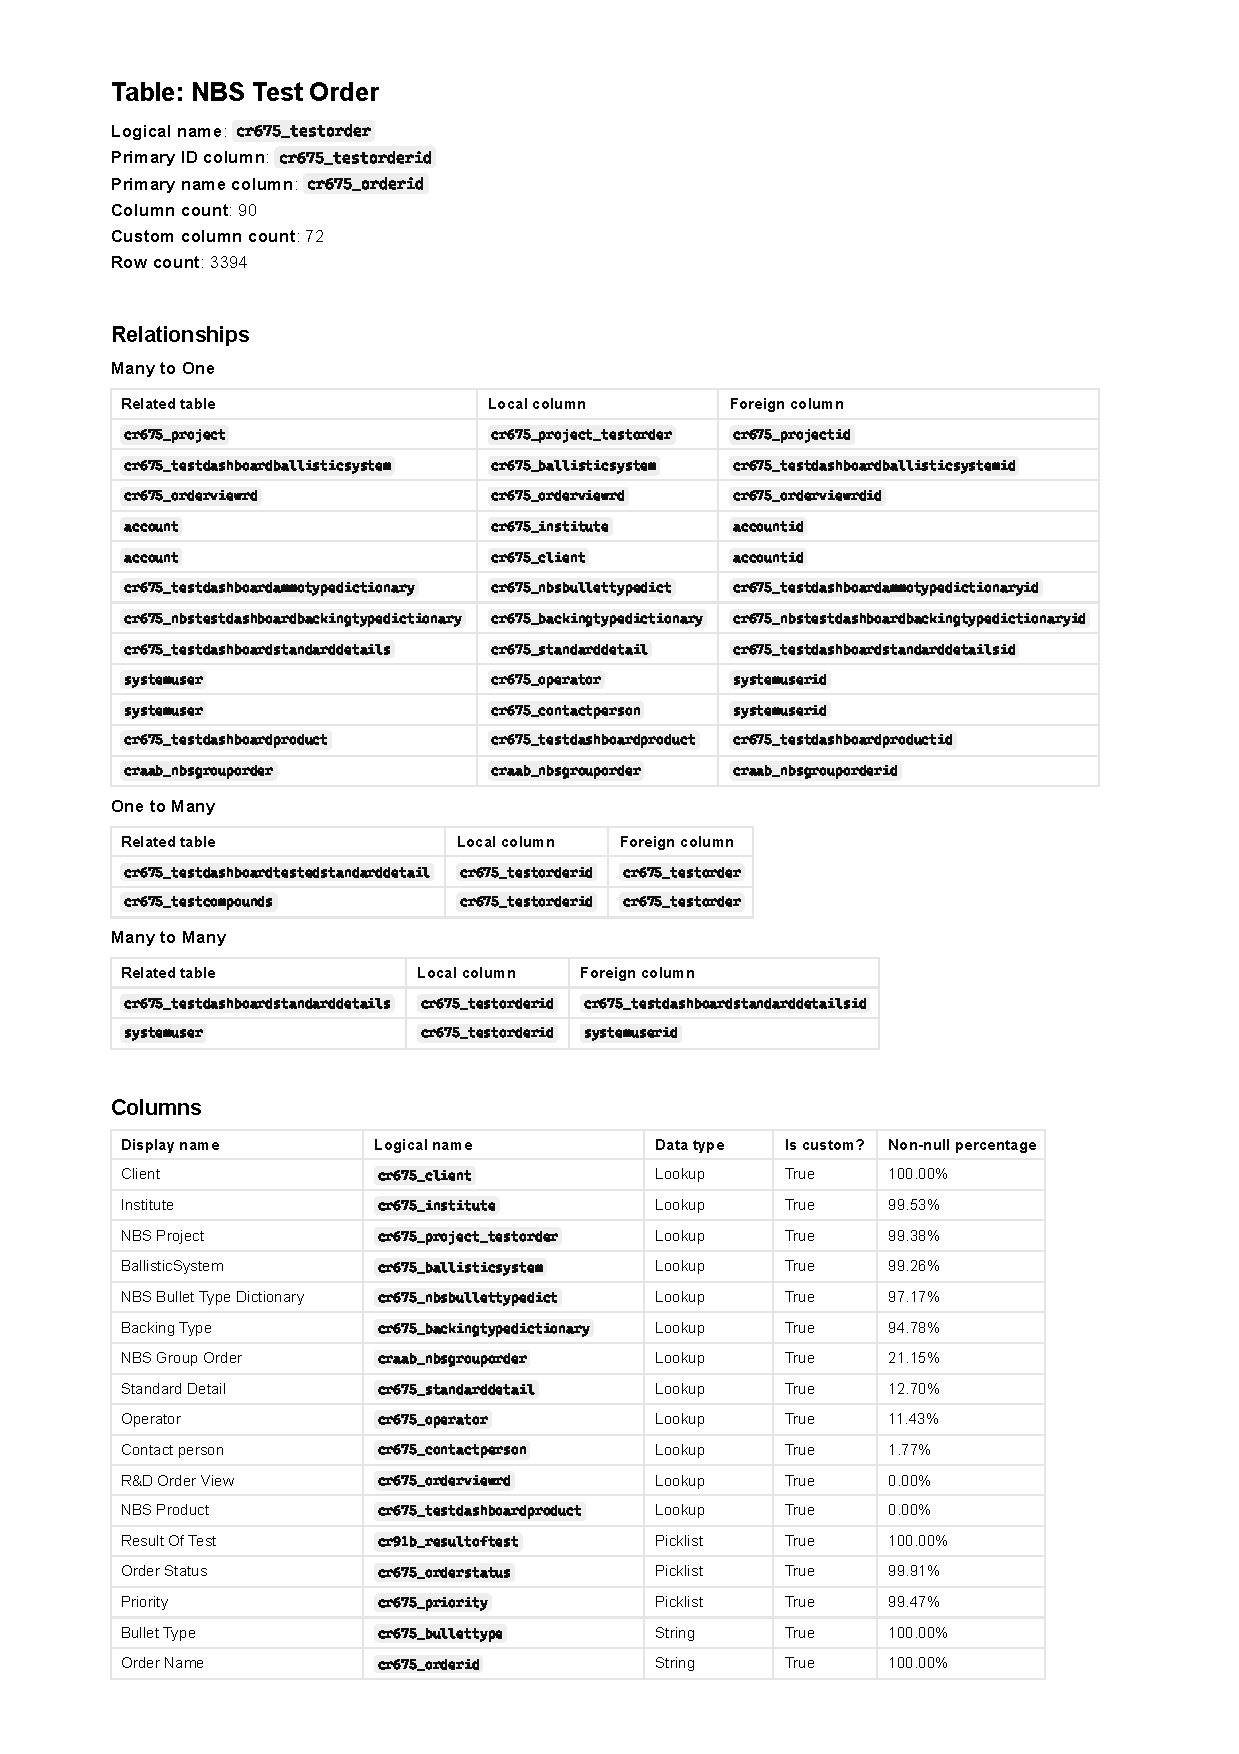
\includepdf[pages=-]{PDFs/tables_markdown.pdf}

\subsection{Solutions}

A \textbf{solution} is a logical container for components such as tables, apps, dashboards, and other resources that are related to a specific process or system. Solutions play a key role in organizing and managing system components, particularly when moving them between environments.

As described by Microsoft:

\begin{quote}
	Solutions are used to transport apps and components from one environment to another or to apply a set of customizations to existing apps. A solution can contain one or more apps as well as other components such as site maps, tables, processes, web resources, choices, flows, and more. \\
	\href{https://learn.microsoft.com/en-us/power-apps/maker/data-platform/solutions-overview}{Source}
\end{quote}

In the context of the NBS system, it was critical to identify which solutions were associated with the system. This information will be essential for migrating the NBS system from the current \texttt{NFM Group Def} environment to the \texttt{NFM Group NBS DEV} environment. Properly identifying and organizing these solutions ensures that all related components—tables, apps, and workflows—are migrated seamlessly.

Each solution has a \textbf{display name} (used for easy identification) and a \textbf{unique name}, which serves as an identifier for system-level operations. This distinction helps ensure that the correct solutions are managed during customization or migration efforts.

\subsubsection{List of Solutions Related to NBS}

\begin{small}
	\begin{tabularx}{\textwidth}{l|l}
		\textbf{Display name} & \textbf{Unique name} \\
		\hline
		Ribbon\_1 & \texttt{Ribbon\_1} \\
		Ribbon\_2 & \texttt{Ribbon\_2} \\
		Ribbon\_3 & \texttt{Ribbon\_3} \\
		Ribbon\_4 & \texttt{Ribbon\_4} \\
		Ribbon\_5 & \texttt{Ribbon\_5} \\
		NBS Product & \texttt{NBSProduct} \\
		NBS Construction & \texttt{NBSConstruction} \\
		Balistic System & \texttt{BalisticSystem} \\
		NBS Geometry & \texttt{NBSGeometry} \\
		NBSTestOrder & \texttt{NBSTestOrder} \\
		NBS Project & \texttt{NBSProject} \\
		NBS PreliminaryTest & \texttt{PreliminaryTest} \\
		Backing Type & \texttt{BackingType} \\
		NBS Model-Driven & \texttt{NBSModelDriven} \\
		NBS Apps & \texttt{NBSApps} \\
		remove dependencies & \texttt{removedependencies} \\
		NBS Migration & \texttt{NBSMigration} \\
		NBS Tester & \texttt{NBSTester} \\
		Construction Creator Model Driven & \texttt{ConstructionCreatorModelDriven} \\
		NBS Database & \texttt{NBSDatabase} \\
		NBS Data Base for migration & \texttt{NBSDataBaseformigration} \\
		NFM BallisticDB & \texttt{NFMBallisticDB} \\
		Account & \texttt{Account} \\
		Common Data Services Default Solution & \texttt{Crb118a} \\
	\end{tabularx}
\end{small}

\subsubsection{Inventory of Solutions Related to NBS}

Below is a comprehensive inventarization of solutions along with their components such as tables and apps.

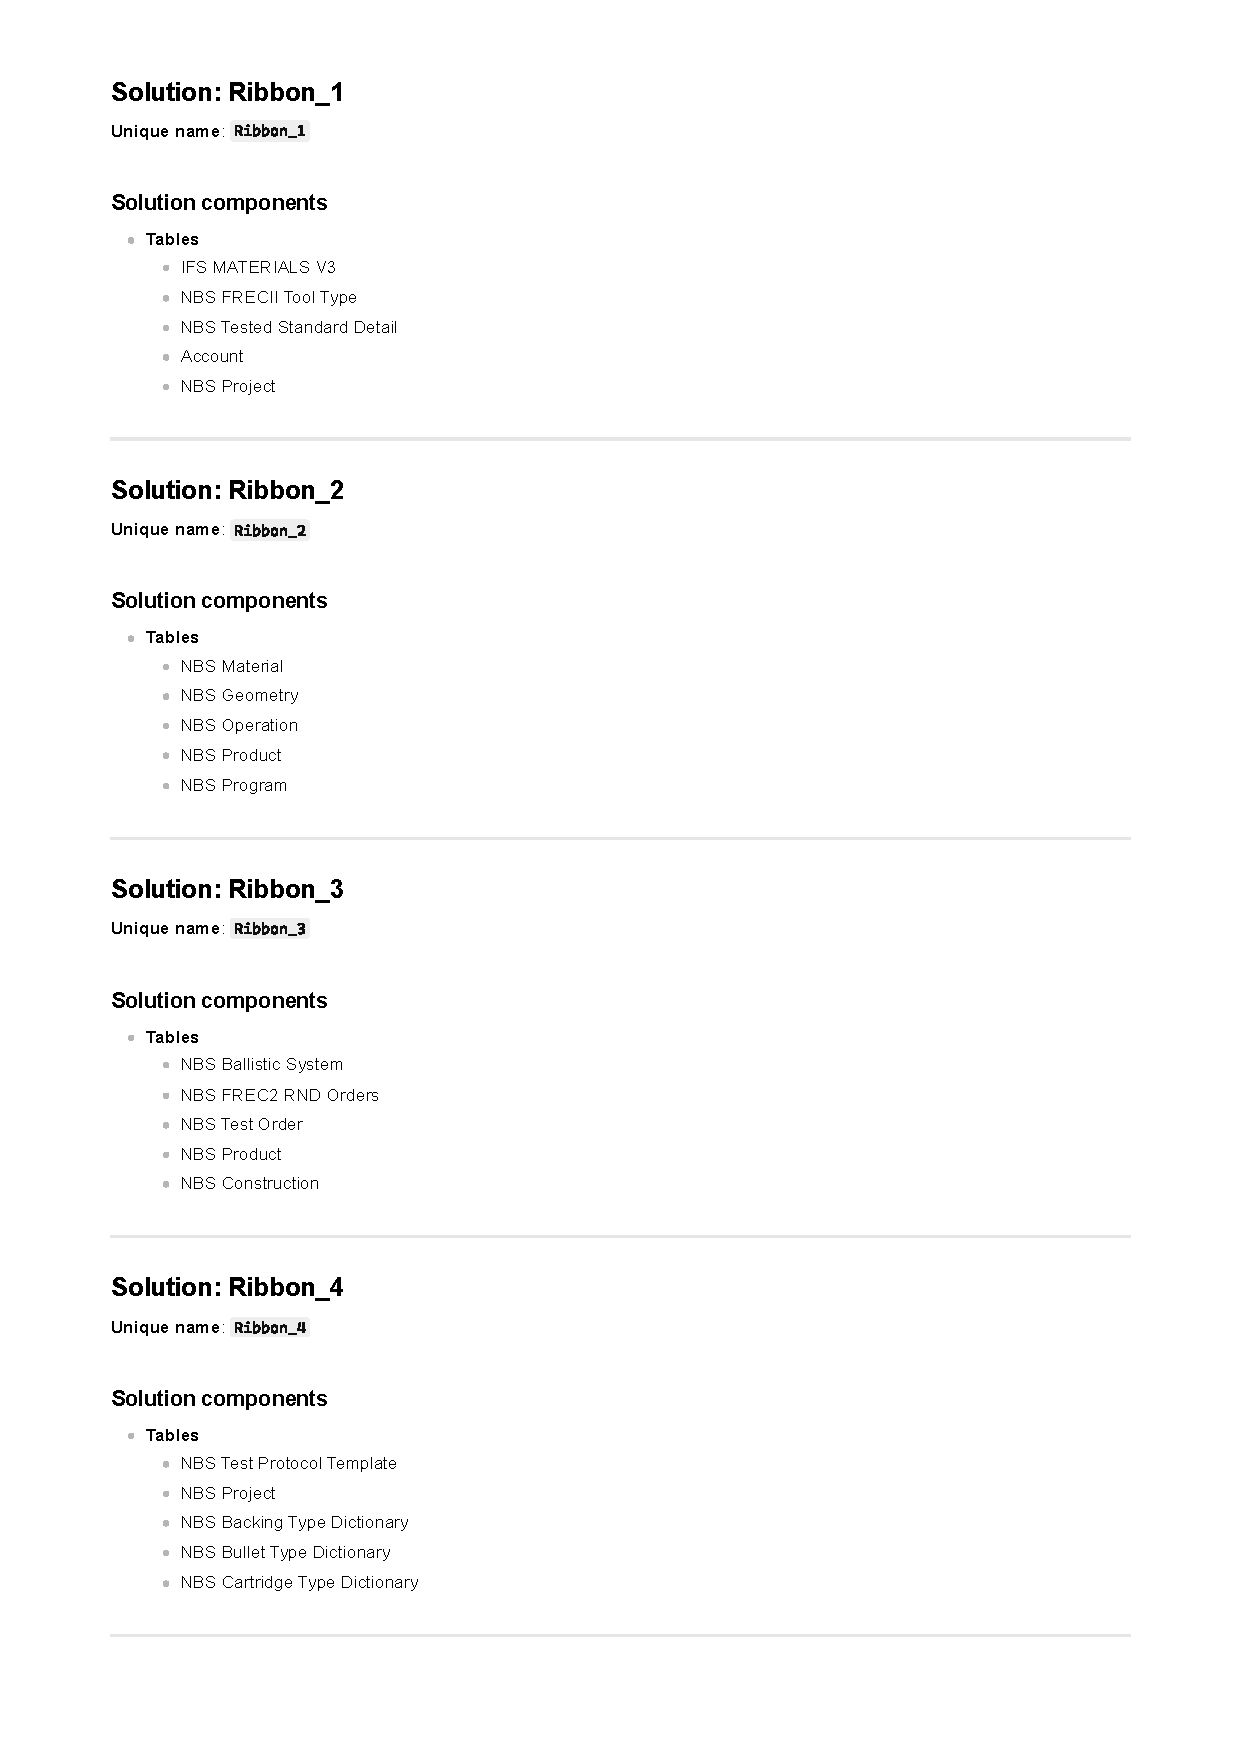
\includepdf[pages=-]{PDFs/solutions_markdown.pdf}

\subsection{Reports}

One of the tasks for this project was to review all of the Power BI Reports used in the \texttt{NBS} Workspace. Each report has been reviewed and described in detail.

Here is a comprehensive inventory of all the reports in the \texttt{NBS} Workspace. Each report contains a description, a list of pages available, filters available, graphs used in the report, and tables used by the report.

\subsubsection{List of Reports Related to NBS}

\begin{small}
	\begin{tabularx}{\textwidth}{l|l}
		\textbf{Report name} & \textbf{Semantic model used} \\
		\hline
		Count of Tested Samples & \texttt{Count of Tested Samples} \\
		Pressed plates count & \texttt{Pressed plates count} \\
		NBS Report Test Range Monitor PL & \texttt{NBS Report\_Test Range Monitor} \\
		NBS Report\_Test Range Monitor & \texttt{NBS Report\_Test Range Monitor} \\
		NBS Report & \texttt{NBS Report} \\
		NBS BSR v1 & \texttt{NBS Report} \\
		NBS Report\_Eabs analysis & \texttt{NBS Report} \\
		NBS Report\_Eabs analysis\_Terje\_cleaned2 & \texttt{NBS Report} \\
	\end{tabularx}
\end{small}

\subsubsection{Inventory of Reports Related to NBS}

This section includes a detailed inventory of all reports related to NBS, including descriptions, pages, filters, and data sources for each report.

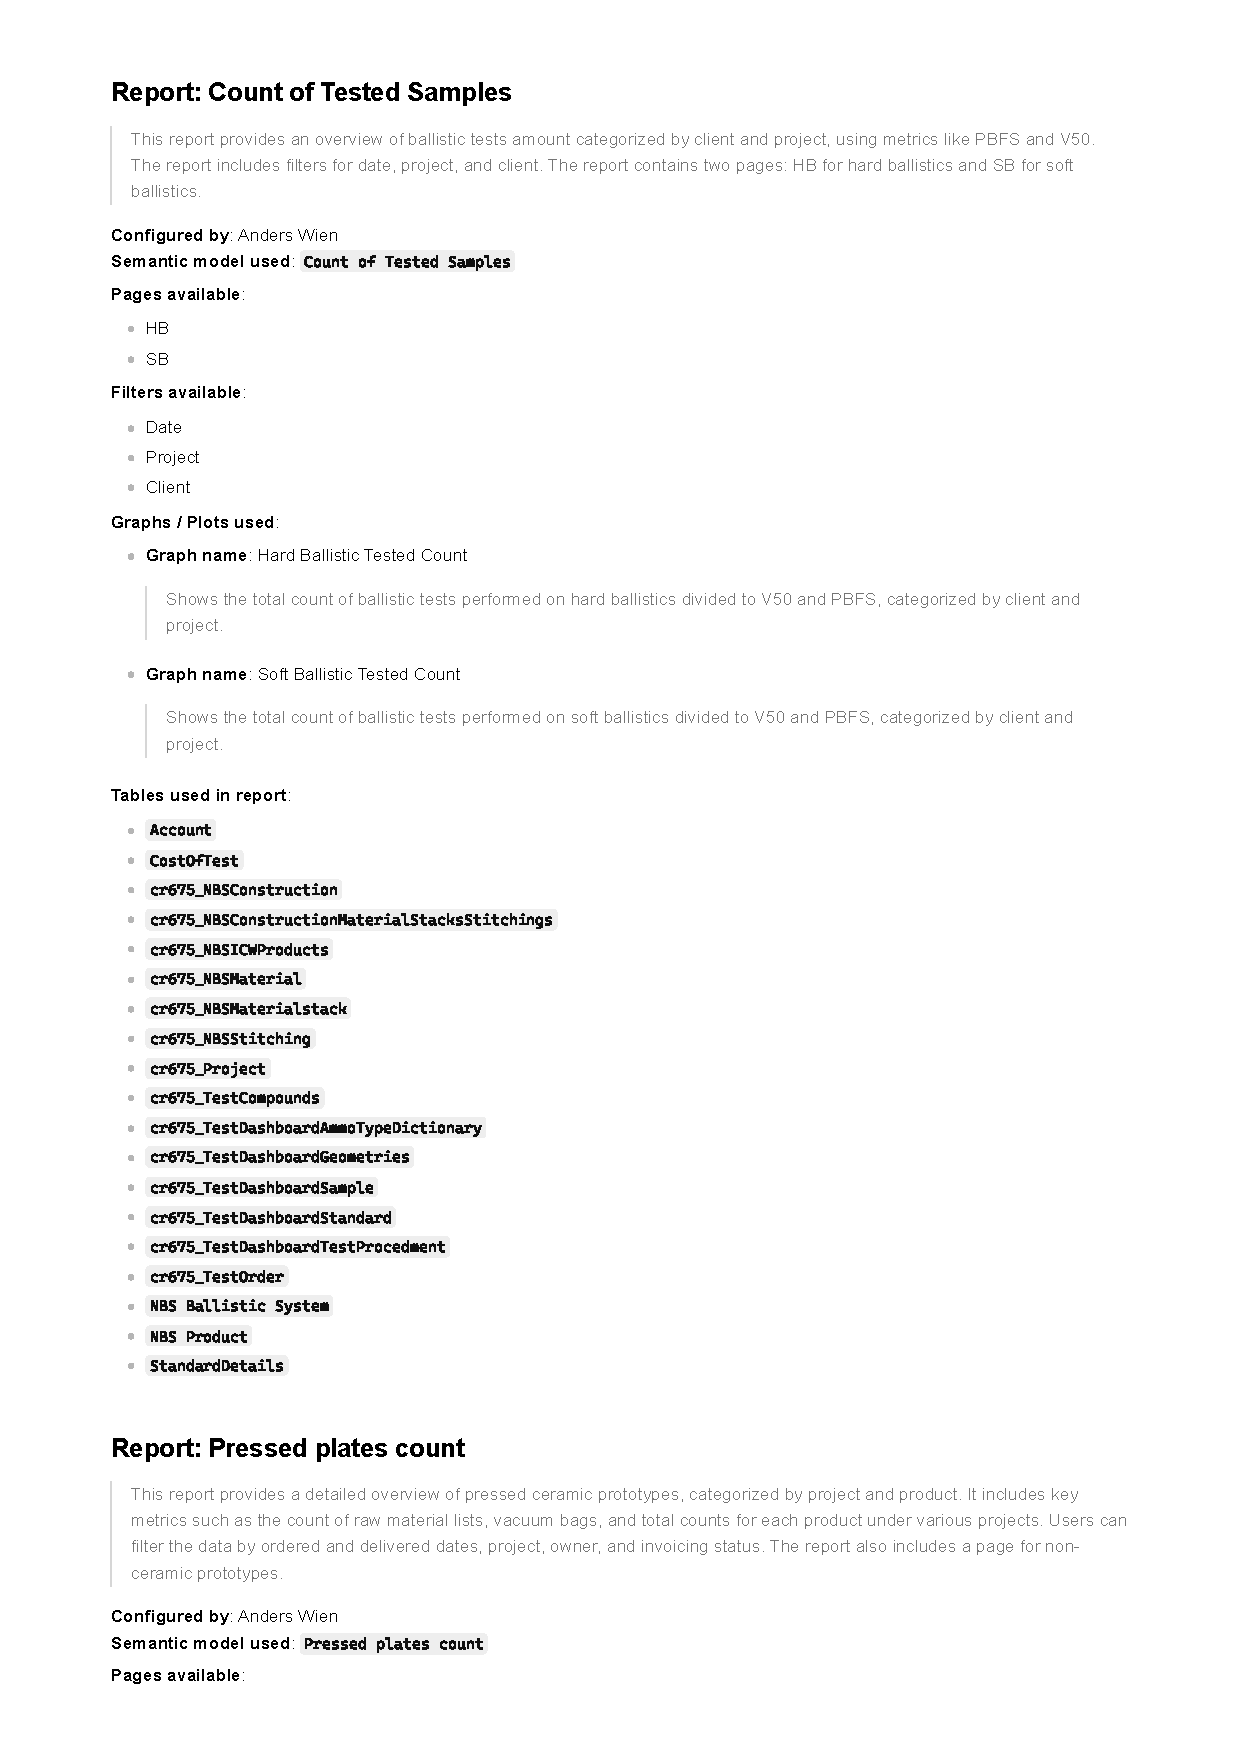
\includepdf[pages=-]{PDFs/reports_markdown.pdf}